\newpage
\section{Инструмент тестов на проникновение Metasploit}

\subsection{Цель работы}

\subsection{Ход работы}

\subsubsection{Описать последовательность действий для получения доступа к консоли}

Атакующая машина (kali linux) -- 192.168.124.210.
Атакуемая машина (Metasploitable2) -- 192.168.124.211.

\paragraph{Подключиться к VNC-серверу, получить доступ к консоли}

% applications > kali linux > system services > metasploit > start

% applications > kali linux > top 10 security tools > metasploit framework

% msfconsole

Для решения этой задачи будем использовать модуль vnc\_login (рис. 3).

\begin{figure}[h!]
\centering
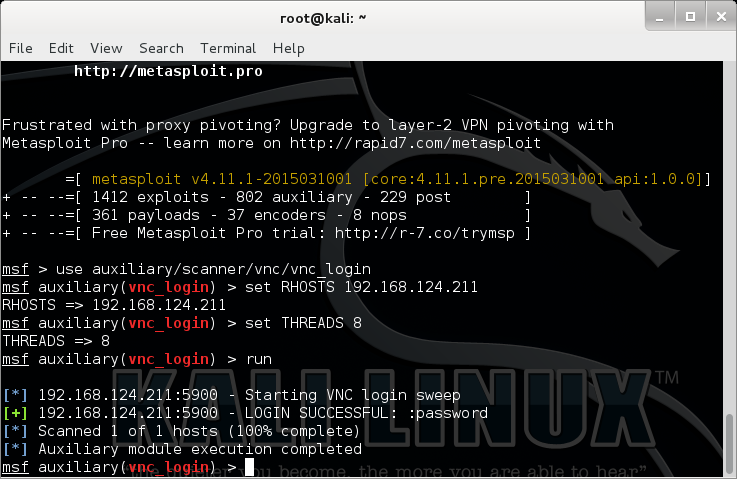
\includegraphics[scale=0.9]{res/pic03}
\caption{Работа с модулем vnc\_login}
\end{figure}

Этот модуль подключается из консоли mfs командой

\begin{Verbatim}[frame=single]
use auxiliary/scanner/vnc/vnc_login
\end{Verbatim}

Выставив параметры RHOSTS и THREADS мы определили целевой компьютер и количество потоков для работы. После чего запустили модуль. Пароль был подобран практически сразу.

НА рисунке 4 показан результат - подключение к VNC-серверу (детали видны в заголовке окна) используя полученный пароль.

\begin{figure}[h!]
\centering
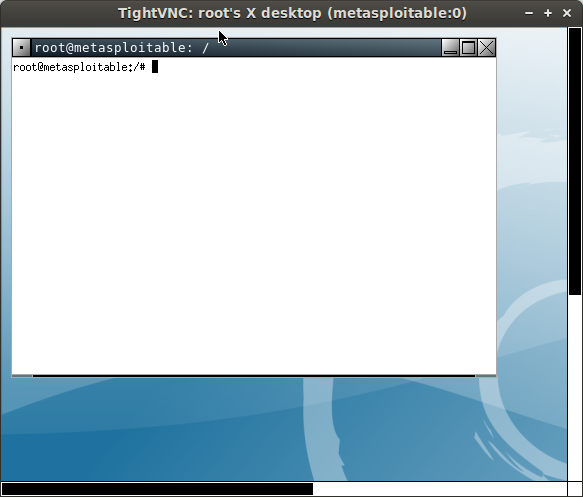
\includegraphics[scale=0.8]{res/pic04}
\caption{Подключение по VNC-протоколу}
\end{figure}

\paragraph{Получить список директорий в общем доступе по протоколу SMB}

Перечислить доступные директории можно при помощи модуля smb\_enumshares.

Этот модуль подключается командой

\begin{Verbatim}[frame=single]
use auxiliary/scanner/smb/smb_enumshares
\end{Verbatim}

Как и в предыдущем случае, для определения целевого хоста и указания количества потоков используются переменные RHOSTS и THREADS соответственно. Результат на рисунке 5. Открыты стандартные ресурсы, видимо используются настройки samba по умолчанию.

\begin{figure}[h!]
\centering
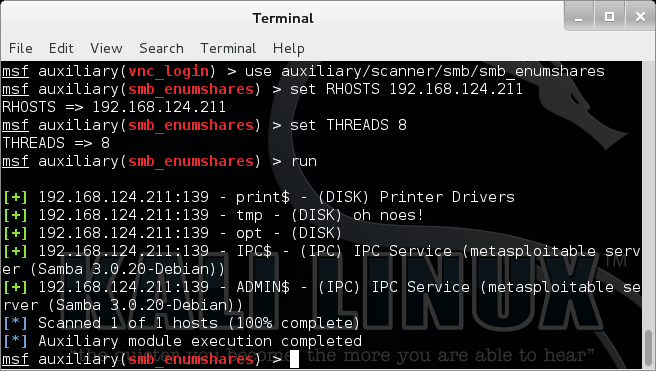
\includegraphics[scale=1]{res/pic05}
\caption{Работа с модулем smb\_enumshares}
\end{figure}


\paragraph{Получить консоль используя уязвимость в vsftpd}

% exploit/unix/irc/unrealircd 3281_backdoor

Для vsFTPd версии 2.3.4, входящего в состав Metasploitable2, уже есть готовый экспоит.

Для начала, его нужно загрузить

\begin{Verbatim}[frame=single]
use exploit/unix/ftp/vsftpd_234_backdoor
\end{Verbatim}

Кроме этого, эксплоит использует набор команд, которые помещены в отдельный файл и их необходимо передать через переменню PAYLOAD. Файл находится по пути cdm/unix/interact, это можно определить используя команду

\begin{Verbatim}[frame=single]
show payloads
\end{Verbatim}

В RHOST записывается доменное имя или IP адрес целевой машины. Запускатся эксплоит командой exploit.

В результатае работы эксплоита, на целевой машине можно получить root-доступ (рисунке 6), что, кроме прочего, говорит о неправильной конфигурации vsFTPd.

\begin{figure}[h!]
\centering
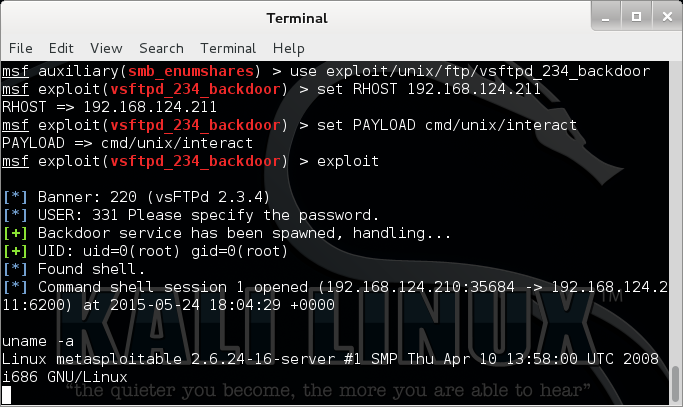
\includegraphics[scale=0.95]{res/pic06}
\caption{Эксплуатация уязвимостей vsFTPd}
\end{figure}

\paragraph{Получить консоль используя уязвимость в irc}

Для решения этой задачи тоже существует эксплоит, называется unreal\_ircd\_3281\_backdoor

\begin{Verbatim}[frame=single]
use exploit/unix/irc/unreal_ircd_3281_backdoor
\end{Verbatim}

Далее требуется устрановить цель и запустить эксплоит (рисунок 7).

\begin{figure}[h!]
\centering
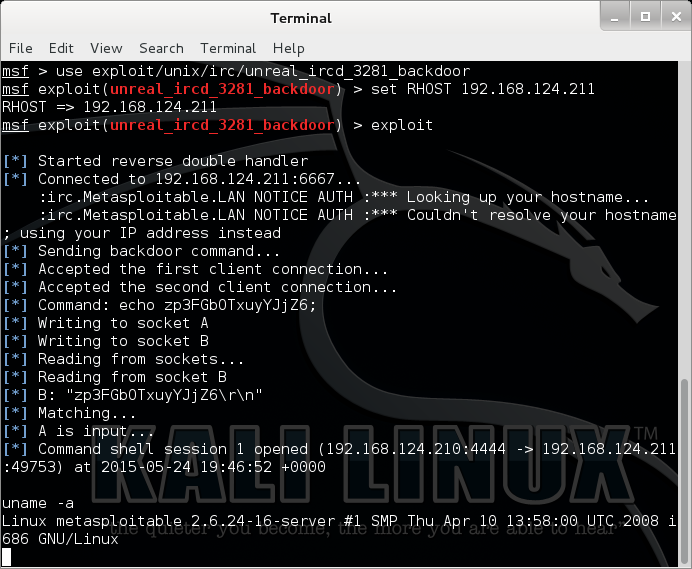
\includegraphics[scale=0.75]{res/pic07}
\caption{Эксплуатация уязвимостей IRC}
\end{figure}

\paragraph{Armitage Hail Mary}

Hail Mary это модуль, поочерёдно запускающий все эксплоиты, которые могут применены к выбранному хосту. В результате (рисунок 8) удалось обнаружить несколько уязвимостей, открывающих доступ к интерпритатору команд.

\begin{figure}[h!]
\centering
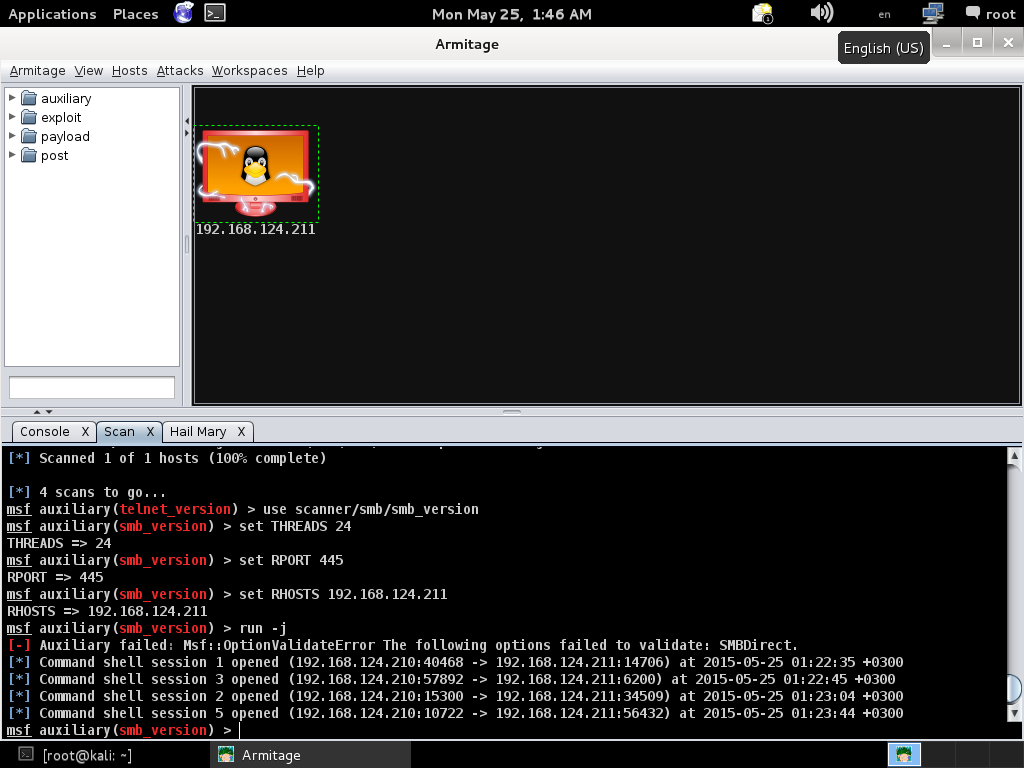
\includegraphics[scale=0.50]{res/pic08}
\caption{Итог работы модуля Hail Mary}
\end{figure}

\newpage
\subsubsection{Изучить три файла с исходным кодом эксплойтов или служебных скриптов на ruby и описать, что в них происходит}

Файл ftp\_version.rb (дистинг 6) описывает попытку получения версии FTP сервера из его банера.

\lstinputlisting[language=Ruby, caption={modules/auxiliary/scanner/ftp/ftp\_version.rb}]{res/ftp_version.rb}

В листинге 7 представлен файл wordpress\_scanner.rb. Он используется для сканирования хоста, выявления CMS WordPress и её версии.

\lstinputlisting[language=Ruby, caption={Файл modules/auxiliary/scanner/http/wordpress\_scanner.rb}]{res/wordpress_scanner.rb}

Файл isc\_dhcpd\_clientid.rb из листинга 8 содержит код, который формирует такой пакет, который выводит из строя DHCP-сервер (ISC DHCP server).

\lstinputlisting[language=Ruby, caption={modules/auxiliary/dos/dhcp/isc\_dhcpd\_clientid.rb}]{res/isc_dhcpd_clientid.rb}

\subsection{Выводы}

Metasploit позволяет конструировать эксплойты с необходимой нагрузкой (payloads), которая выполняется в случае удачной атаки, например, установка shell или VNC сервера. Также фреймворк позволяет шифровать шеллкод, что может скрыть факт атаки от IDS или IPS. Для проведения атаки необходима информация об установленных на удаленном сервере сервисах и их версии, то есть нужно дополнительное исследование с помощью таких инструментов, как nmap.